\section{Aufbau der W"armepumpe}
\label{sec:aufbau}
	\begin{wrapfigure}{r}{8cm}
		\centering
		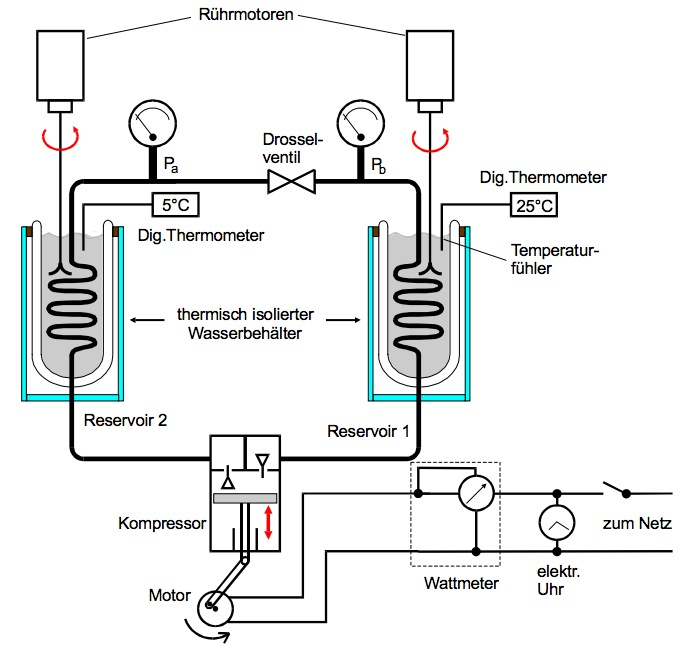
\includegraphics[width = 8cm]{img/pumpe.jpeg}
		\caption{Schemenhafter Aufbau der verwendeten W"armepumpe \label{fig:pumpe}}
	\end{wrapfigure}

	Im Folgenden wird der Aufbau einer W"armepumpe erl"autert.
	Abbildung \ref{fig:pumpe} skizziert den Aufbau der hier verwendeten Apparatur. \\

	Um eine W"armepumpe zu realisieren, benutzt man zun"achst als Transportmedium ein Gas, das beim Verdampfen W"arme aufnimmt und diese beim Kondensieren wieder abgibt.
	Die beiden W"armereservoirs sind durch Rohre verbunden, in denen das Gas flie"sen kann.
	Es wird durch einen Kompressor zwischen den Reservoirs bewegt.

	Ein Drosselventil sorgt daf"ur, dass sich auf einer Seite des Ventils ein Druck $p_\mathrm{b}$ aufbaut.
	Auf dieser Seite befindet sich das zu w"armende Reservoir 1, welches die Temperatur $T_1$ besitzt.

	Am Ventil f"allt der Druck ab, sodass auf der Seite von Reservoir 2 (mit Temperatur $T_2$) ein geringerer Druck $p_\mathrm{a}$ herrscht.

	Mit der Durchl"assigkeit des Ventils lassen sich die beiden Dr"ucke $p_\mathrm{a}$ und $p_\mathrm{b}$ so steuern, dass das Transportmedium im Reservoir 2 in den gasf"ormigen Zustand wechselt und dabei die W"armemenge $Q_2$ aufnimmt.

	Das aufgew"armte Gas wird dann durch den Kompressor in den Bereich des h"oheren Druckes $p_\mathrm{b}$ gepresst.
	Wenn es dort durch Reservoir 1 geleitet wird, kondensiert es, wobei die zuvor aufgenommene W"armemenge $Q_2$ wieder abgegeben wird.
	Das Medium durchl"auft anschlie"send das Drosselventil und der Prozess beginnt von Neuem.

	Somit wird dem Reservoir 1 sukzessive W"arme aus Reservoir 2 zugef"uhrt. \\


	Die Dr"ucke $p_\mathrm{a}$ und $p_\mathrm{b}$ lassen sich beim hier verwendeten Aufbau duch Manometer ablesen.
	Jedes Reservoir besteht aus einem thermisch isolierten Wasserbeh"alter, dessen Wassertemperatur mit Hilfe von Thermometern abgelesen werden kann.
	Zudem sorgen R"uhrmotoren f"ur eine st"andige Durchmischung des Wassers.

	Die Leistung des Kompressors kann ebenfalls mittels eines Wattmeters abgelesen werden.
	
\clearpage
\section{Durchf"uhrung}
\label{sec:durchfuehrung}
	Zun"achst werden die Wasserbeh"alter mit einer bestimmten Wassermenge $m$ gef"ullt.
	Der Kompressor wird eingeschaltet und es werden die Werte der Dr"ucke $p_\mathrm{a}$ und $p_\mathrm{b}$, die Temperaturen $T_1$ und $T_2$, sowie die Leistungsaufnahme $W$ des Kompressors in Abh"angigkeit von der Zeit $t$ gemessen.
	Beim hier verwendeten Gas handelt es sich um Dichlordifluormethan. \\

	Aus den Messdaten soll dann die reale G"uteziffer $\nu$ bestimmt werden.
	Mit Hilfe des Differenzenquotienten der Temperatur $T_1$ zur Zeit $t$ l"asst sich $\nu$ durch Ausgleichsrechnung ermitteln. Es gilt
	\begin{equation}
		\nu = (m_1 c_\mathrm{W} + m_\mathrm{k} c_\mathrm{k}) \frac{\Delta T_1}{\Delta t} \frac{1}{W} \,,
	\end{equation}

	wobei $m_1 c_\mathrm{W}$ die W"armekapazit"at des Wassers, $M_\mathrm{k} c_\mathrm{k}$ die W"armekapazit"at des Gef"a"ses mit Kupferrohr und $W$ die zeitlich gemittelte Leistung des Kompressors bezeichnet. \\

	Anschlie"send wird der Massendurchsatz $\Delta m / \Delta t$ des Transportmediums berechnet.
	Bei der Verdampfung des Mediums wird pro Zeit und Masse die Verdampfungsw"arme $L$ verbraucht und es gilt
	\begin{equation}
		(m_2 c_\mathrm{W} + m_\mathrm{k} c_\mathrm{k}) \frac{\Delta T_2}{\Delta t} = L \frac{\Delta m}{\Delta t} \,.
	\end{equation}

	Schlie"slich soll die mechanische Kpmpressorleistung $W_\mathrm{m}$ bestimmt werden.
	Durch Integration des Druckes im Kompressor und Hinzunahme der Poissonschen Gleichung l"asst sich diese Bestimmen.
	Mit $\kappa$, dem Verh"altnis der Molw"armen $c_\mathrm{p}$ und $c_\mathrm{v}$ sowie $\rho$, der Dichte des Transportmediums gilt
	\begin{equation}
		W_\mathrm{m} = \frac{1}{\kappa -1} \left[p_\mathrm{b} \left(\frac{p_\mathrm{a}}{p_\mathrm{b}}\right)^\frac{1}{\kappa} - p_\mathrm{a}\right] \frac{1}{\rho}\frac{\Delta m}{\Delta t} \,.
	\end{equation}